\documentclass[11pt]{article}

\usepackage{amsmath, amssymb, amsfonts, amsthm}
\usepackage{hyperref}
\usepackage{mathtools}
\usepackage{centernot}
\usepackage{fancyhdr}
\usepackage{fancyvrb}
\usepackage{verbatim}
\usepackage{xcolor}
\usepackage{enumerate}
\usepackage{tikz}
\usepackage{gensymb}
\usepackage{booktabs}
\usepackage{multirow}
\usepackage{siunitx}
\usepackage[margin=0.9in,includefoot]{geometry}
\usepackage{graphicx}
\graphicspath{ {images/} }
\usepackage{longtable}
\usepackage[export]{adjustbox}
\usepackage{setspace}
\usepackage{array}
\usepackage{chngcntr}
\usepackage{pbox}
\usepackage{calc}
\usepackage{hyperref}
\usepackage{extramarks} % Required for headers and footers
\usepackage{listings,relsize}
\usepackage{csquotes}
\usepackage[shortlabels]{enumitem}
\usepackage{fancyhdr}
\usepackage{apacite}

% setup other parameters
\lstloadlanguages{R}
\pagestyle{fancy}
\fancyhf{}
\newcommand{\lil}[1]{\lstinline|#1|}
\renewcommand{\sectionmark}[1]{\markright{\thesection\ #1}}
\fancyhead[RO]{\thepage}
\pagenumbering{roman}
\counterwithin{figure}{section}
\counterwithin{table}{section}

% setup hyperlink format
\hypersetup{
  colorlinks,
  linkcolor=wine-stain,
  linktoc=all
}

% setup lstlisting format
\definecolor{wine-stain}{rgb}{0.5,0,0}
\lstdefinestyle{base}{
  language=Matlab,
  emptylines=1,
  breaklines=true,
  basicstyle=\ttfamily\color{black},
  moredelim=**[is][\color{blue}]{@}{@}
}



\begin{document}

% title page
\begin{titlepage}
   \begin{center}
   \line(1,0){450}\\
   [0.25in]
   \huge{\bfseries Applications of Supervised and Semi-supervised Machine Learning Algorithms on Forest Cover Type Classification Problem}\\
   [2mm]
   \line(1,0){450}\\
   [0.5cm]
   \textsc{\begin{large}
   Department of Statistics and Actuarial Science\\
   University of Waterloo\\
   WINTER 2015 STAT 441
   \end{large}}\\
   \textsc{\begin{normalsize}
   \end{normalsize}}\\
   \begin{normalsize}
		\textbf{Yilun Zhang} $\cdot$ \texttt{20422438} $\cdot$ \texttt{yl5zhang@uwaterloo.ca}\\
		\textbf{Yanbing Jin} $\cdot$ \texttt{20412945} $\cdot$ \texttt{y36jin@uwaterloo.ca}\\
		[2cm]
   \end{normalsize}

% abstract
\begin{abstract}
\noindent\large\onehalfspacing
This report summarized supervised and semi-supervised machine learning algorithms being applied to predict the predominant forest cover type in a Kaggle competition. The analysis flow includes exploratory data analysis, dimensionality reduction, supervised model fitting including logistic regression, tree based ensemble learning methods, gradient boosting, adaptive boosting, naive bayes, support vector machine and neural network, feature creation and selection, semi-supervised learning algorithm using graph based label spreading and propagation. Classification error rate was used to measure model accuracy. The best performing model is the extremely randomized tree model with grid searched parameters fitting on data with 116 features selected from features including base, 2-way and 3-way interactions by gini variable importance. This model resulted in rank 362 among all 1694 teams participated in this Kaggle competition.
\end{abstract}

\end{center}
\end{titlepage}

% table of content
\tableofcontents
\thispagestyle{empty}
\cleardoublepage


% main paragraphs start here
\newpage
\setcounter{page}{1}
\pagenumbering{arabic}


% set line spacing to be 1.5
% \onehalfspacing
\singlespace

% introduction
\section{Data and Problem}

The forest cover type classification problem is a past Kaggle competition held from May 2014 to May 2015 (\href{https://www.kaggle.com/c/forest-cover-type-prediction}{https://www.kaggle.com/c/forest-cover-type-prediction}). In this competition, competitors were asked to used the provided data to predict the predominant forest cover type. \\

\noindent Data is taken from Roosevelt National Forest of Northern Colorado and provided by US Geological Survey (USGS) and US Forest Service (USFS). It contains 15,120 training samples and 565,892 testing samples. Each sample represents a 30m by 30m patch in the forest. The goal of the competition is to predict what kind of tree type covers the majority of a patch. \\

\noindent The provided data contains 12 independent variables that are strictly cartographic. These are:
\begin{itemize}
\setlength\itemsep{0cm}
\item Numerical
\begin{itemize}
\setlength\itemsep{0cm}
\item Elevation
\item Aspect
\item Slope
\item Horizontal / Vertical distance to hydrology
\item Horizontal distance to Road
\item Horizontal distance to Wildfire ignition points
\item Hill shade at 9AM / 12PM / 3PM
\end{itemize}
\item Categorical
\begin{itemize}
\setlength\itemsep{0cm}
\item Wilderness area designation (4 types)
\item Soil type (40 types)
\end{itemize}
\end{itemize}
Detailed wilderness area designation and soil type information (i.e. name) can be found from the link provided above. The categorical variables are coded into binary columns. For example, Wilderness area designation takes 4 columns, each represents a type of designation. For each row, the column that contains one of the wilderness are designations will coded as 1, and 0 otherwise.\\

\noindent There are seven types of trees and they are labeled 1 through 7 in the given data set. These are:
\begin{itemize}
\setlength\itemsep{0cm}
\item Spruce/Fir (1)
\item Lodgepole Pine (2)
\item Ponderose Pine (3)
\item Cottonwood/Willow (4)
\item Aspen (5)
\item Douglas-fir (6)
\item Kurmmholz (7)
\end{itemize}

\newpage

\section{Exploratory Data Analysis}
We started off with exploratory analysis to understand the structure of the data and each predictor's distribution and relationship with the label.

\begin{figure}[h]
\label{eda1}
\begin{center}
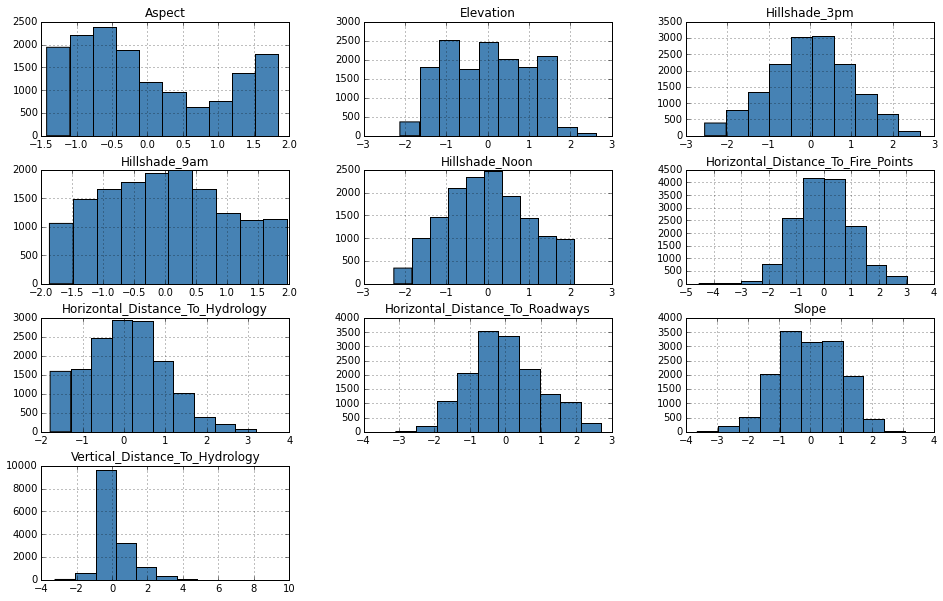
\includegraphics[scale=0.4]{hist.png}
\end{center}
\caption{Histogram of all numerical variables}
\end{figure}

\noindent Figure 2.1 shows the histograms of all numerical variables. We can see that all variables have different distributions, some are left skewed (\texttt{Horizontal\_Distance\_To\_Roadways}), some are right skewed (\texttt{Hillshade\_Noon}), some are bimodal (\texttt{Aspect}). We also noticed that variables take values in various numerical ranges. These suggest potential needs to transform and normalize the given data since a number of machine learning algorithms require/suggest the data to be normalized. In later sections we will fit models on both raw and transformed data to compare model accuracies.

\begin{figure}[h] 
\label{eda2}
\begin{center}
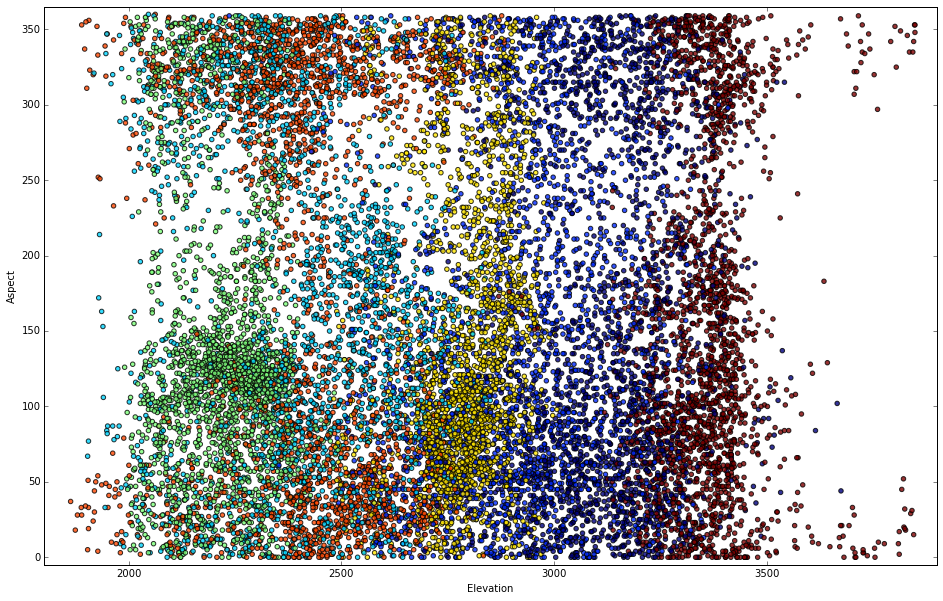
\includegraphics[scale=0.3]{elevation_aspect_vs_label.png}
\end{center}
\caption{Elevation vs. Aspect colored by label}
\end{figure}

\noindent Figure 2.2 shows the scatter plot between \texttt{Elevation} and \texttt{Aspect}, colored by label. We notice that as elevation goes up, though there are some overlaps, the cover type of the patch changes. This indicates that elevation is potentially a good predictor for cover type. Where as in Figure 2.3, we are not able to find clear clusters of points with same label. We need to further investigate these variables in order to see their relationship with the label.

\begin{figure}[h]
\label{eda3}
\begin{center}
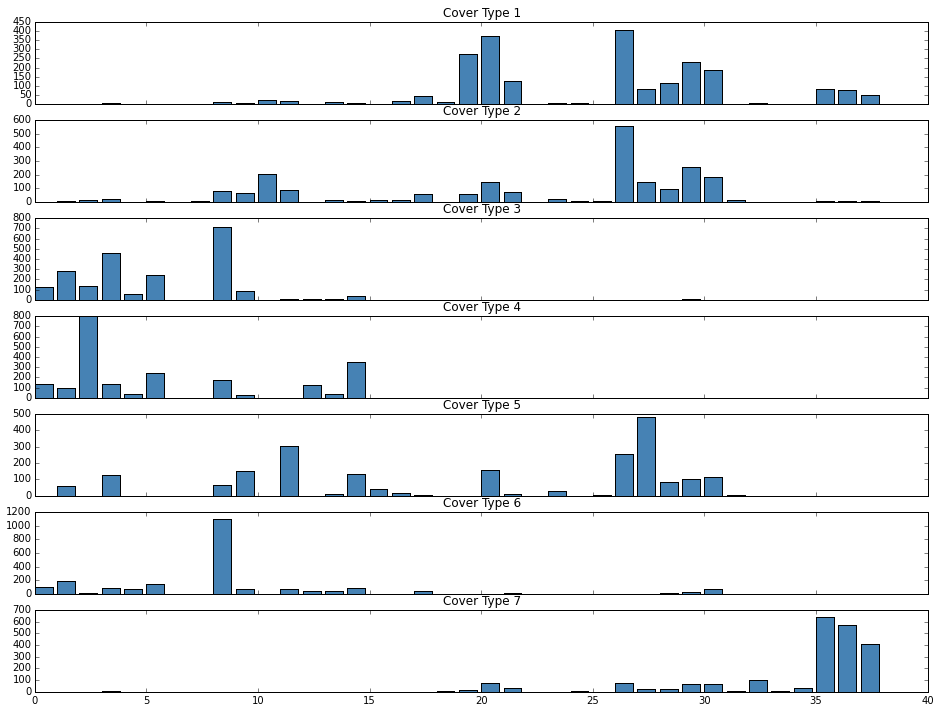
\includegraphics[scale=0.3]{soil_label.png}
\end{center}
\caption{Soil type vs. label}
\end{figure}

\noindent Figure 2.3 shows the distribution of \texttt{Soil\_Type} by \texttt{Cover\_Type}. We can see that for cover label 7, the predominant soil types are 36, 37 and 38 where no other soil type has a predominant soil type of these three. Similarly, soil type 20, 21, 22 are highly related to cover type 1. This suggests \texttt{Soil\_Type} is a good predictor for the label. We can deduce similar insights from Figure 2.4 as well. For example. cover type 4 only exists when the patch is within wilderness designation 4.

\begin{figure}[h]
\label{eda4}
\begin{center}
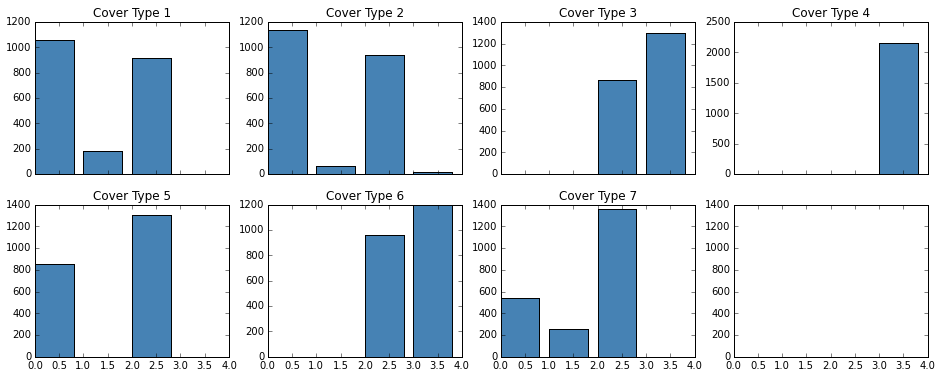
\includegraphics[scale=0.4]{wilderness_label.png}
\end{center}
\caption{Wilderness type vs. label}
\end{figure}

\noindent The distribution of labels (i.e. \texttt{Cover\_Type} is very uniform with each label having 2,160 samples. We do not need to worry about imbalance samples in our case.

\newpage

\section{Dimensionality Reduction}

We proposed two methods for dimensionality reduction to find out whether data can be easily separated in lower dimensions: Principal Component Analysis and Fischer's Linear Discriminant Analysis. If data is separable, we would continue fitting model on these lower dimensions. If not, we will use original matrix for model fitting.

\subsection{Principal Component Analysis (PCA)}
PCA is a dimensionality reduction technique which uses orthogonal transformation to convert original data set to a set of linearly independent principal components. The first component represents the direction that has the highest variance in the dataset. The second component represents the direction that is orthogonal to the first, and explains the next highest variance in the dataset. The idea is to use Singular-Value-Decomposition on normalized matrix:
$$X = U\Sigma V^*$$
where:
\begin{itemize}
\setlength\itemsep{0cm}
\item $U$ is eigenvectors of $X^TX$
\item $V$ is eigenvectors of $XX^T$
\item $\Sigma$ is a diagonal matrix such that diagonal values are the eigen values of $X^TX$ or $XX^T$.
\end{itemize}
To get the first $p$ component, we simply do:
$$U[:,1:p]\Sigma[1:p,1:p] V[:,1:p]^*$$

\noindent Figure 3.1 shows the first 2 and 3 components colored by label. We can hardly separate the colors in these 2 or 3 dimensions, which means PCA is not that beneficial to our data.

\begin{figure}[h]
\label{pca}
\begin{center}
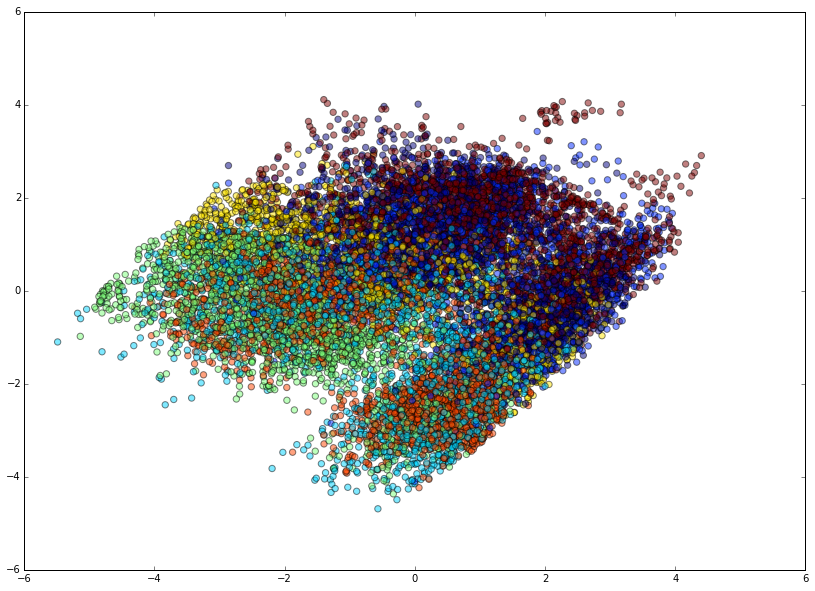
\includegraphics[scale=0.265,valign=t]{pca_2d.png}
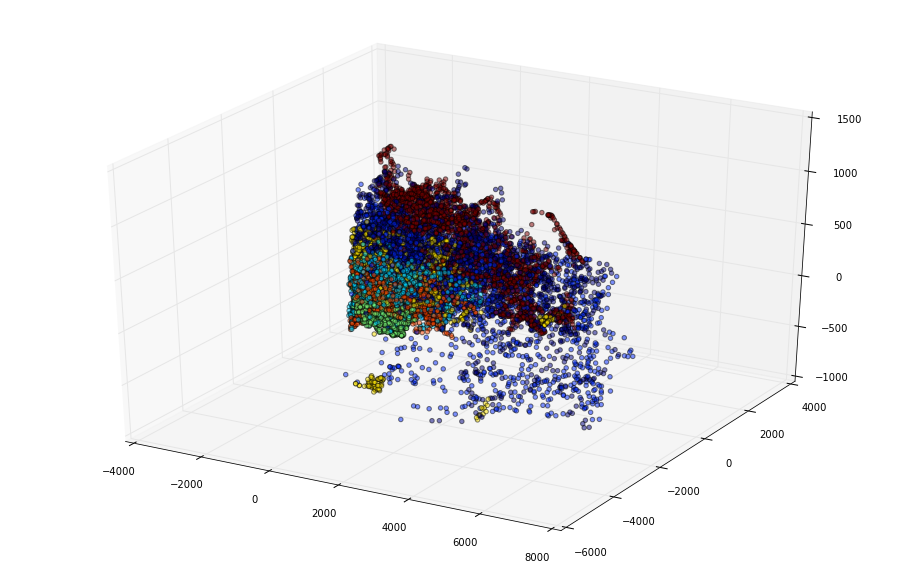
\includegraphics[scale=0.265,valign=t]{pca_3d.png}
\end{center}
\caption{PCA 2D $\&$ 3D}
\end{figure}

\subsection{Fischer's Discriminant Analysis (LDA)}
LDA, different from PCA, finds a linear combination of features that best separates different classes. This means, it also takes the label of each sample into calculation.

\begin{figure}[h]
\label{lda}
\begin{center}
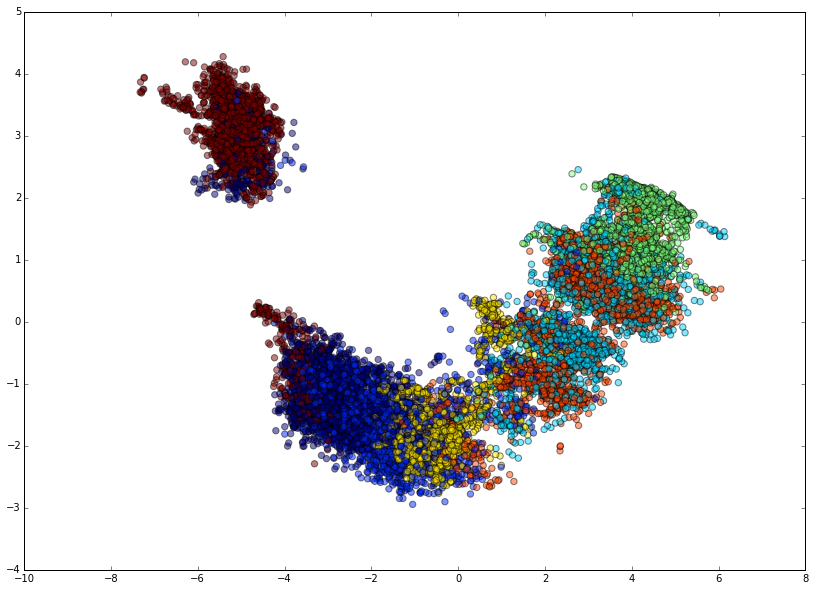
\includegraphics[scale=0.265,valign=t]{lda_2d.png}
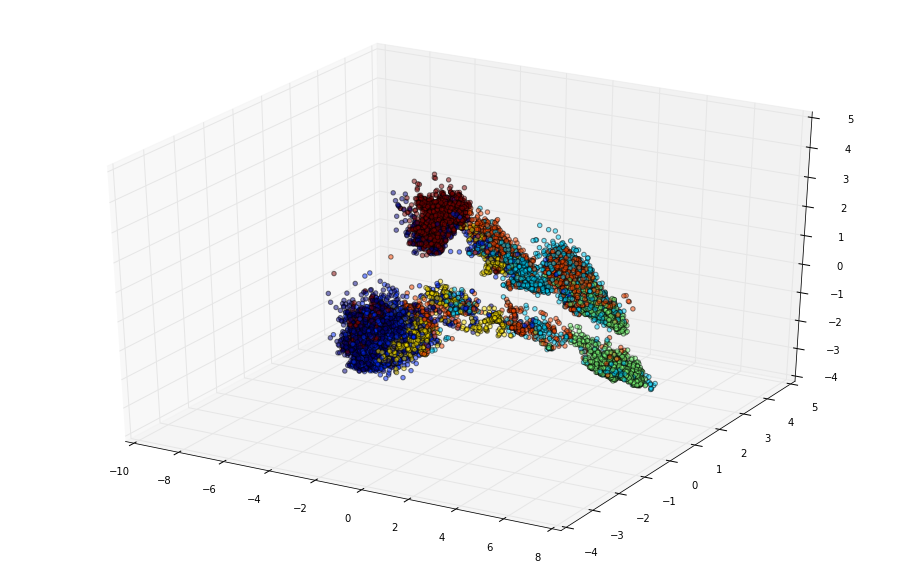
\includegraphics[scale=0.265,valign=t]{lda_3d.png}
\end{center}
\caption{PCA 2D $\&$ 3D}
\end{figure}

\noindent From Figure 3.2 we can some clusters of labels in the 2D case where similar colors are closer to each other and more separable than PCA. However, we still have color blue and red overlapping together and none of the colors are separable by a linear/non-linear line. This is the same for the 3D case and we decided not to use dimension reduced data for model fitting.

\newpage 

\section{Supervised Learning Methods}
After some exploratory analysis on the data and attempting a few dimensionality reduction techniques, we move on to fit machine learning models on our original data. Figure 4.1 shows the basic analysis flow. 

\begin{figure}[h]
\label{flow}
\begin{center}
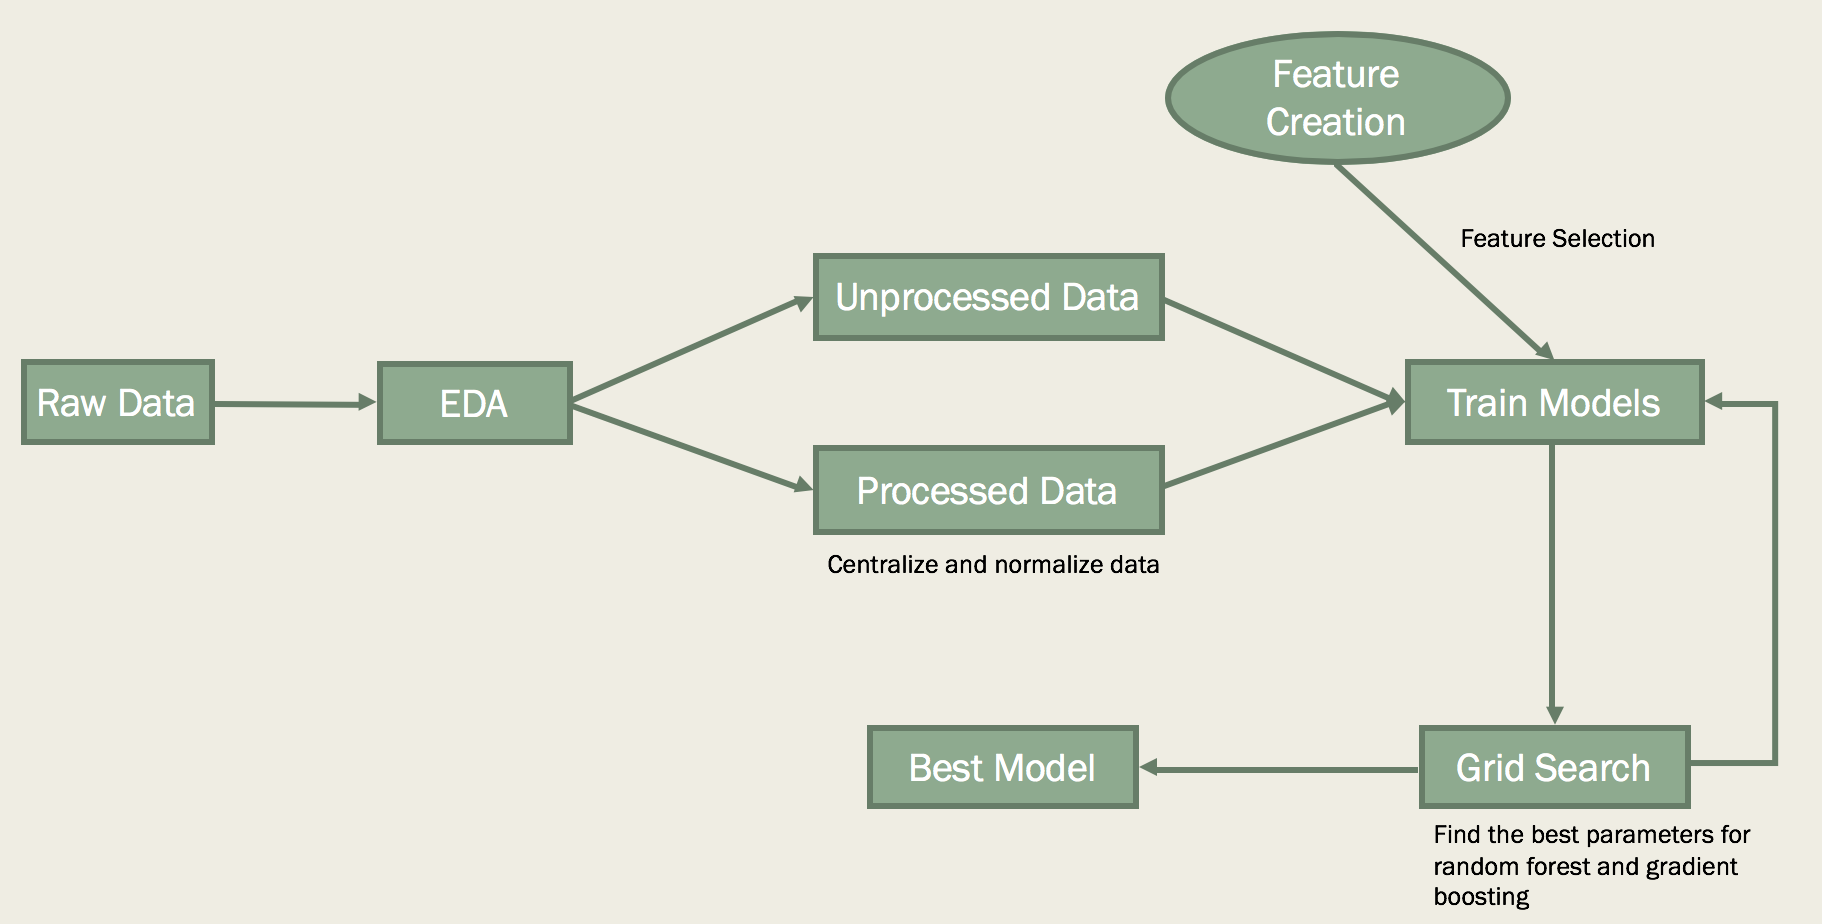
\includegraphics[scale=0.5]{flow.png}
\end{center}
\caption{Analysis Flow}
\end{figure}

\noindent We will proceed to fit default models on both transformed (i.e. normalized, and power transformed) data and raw data for comparison. Models we tried include:
\begin{itemize}
\setlength\itemsep{0cm}
\item Multi-class Logistic Regression (LR)
\item Decision Tree - (DT)
\item Random Forest - (RF)
\item Extremely Randomized Trees - (ERT)
\item Gradient Boosting (Trees) - (GB)
\item Support Vector Machine - (SVM)
\item Gaussian Naive Bayes (GNB)
\item Adaptive Boosting - (AB)
\item Neural Network - (NN)
\end{itemize}
We then chose RF and ERT as candidate models and arid search to find the optimal parameters that minimized the error rate. \\

\noindent Furthermore, we employed feature creation and feature selection techniques to include 2-way and 3-way interaction terms between numerical variables, and used feature importance to select significant features to fit the model. 

\subsection{Advantages and Disadvantages of Each Model}
Before we fit model, we did some research and summarized the advantages and disadvantages of each model we attempt to use.

\begin{enumerate}[(1)]
\setlength\itemsep{0cm}
\item \textbf{Logistic Regression} works great when the labels are linearly separable and it trains and predicts very fast. It is less prone to over-fitting and has easy implementation and interpretation. We can also assess variable importance for model optimization.

\item \textbf{Decision Tree} trains very fast and works good with categorical variables. However since only one tree is fit and if the tree goes too deep, it might overfit the training data.

\item \textbf{Random Forest} is a bootstrap aggregation model that trains a number of decision trees and take the average over them for the final fitting and prediction. On each iteration, it samples the original data set with replacement and fit a new tree. This fixes the overfitting problem that might be caused by fitting a single decision tree. However, since we introduced bootstrap sampling and when fitting the tree, it selects a random subset of the features, it is very difficult to interpret the model.

\item \textbf{Extremely Randomized Trees} is similar to random forest in the content of techniques being used and the issue of overfitting. The difference is that "instead of looking for the most discriminative thresholds, thresholds are drawn at random for each candidate feature and the best of these randomly-generated thresholds is picked as the splitting rule" (Scikit-Learn, 2015).

\item \textbf{Gradient Boosting (Trees)} is a boosting algorithm that fits single decision tree at each iteration. Instead of averaging over all the trees, GB tries to find the best linear combination of fitted trees to explain the training data. As a result of this optimization, the GB model trains much slower but might yields better results. However it is also known to possibly overfit the training data.

\item \textbf{Support Vector Machine} can model complex non-linear relationship in our data and is it robust to noise. On the other hand, SVM model trains very slowly and it is hard to tune parameters. Moreover, it is like a black box and very difficult to interpret the model.

\item \textbf{Adaptive Boosting} model performs extra tuning on weak classifiers and adjust weightings to yield best outcome. It is fast and easy to implement. However it is very sensitive to noise data, if the weak classifiers are too weak or too complex, we might overfit the training data.

\item \textbf{Neural Network} works good on data with non-linear relationship, i.e. image data, sound data. It usually yields good result but it takes a long time to fit and it is very difficult to interpret the model. It requires a large number of training data in order to get good result and estimates a large number of parameters.
\end{enumerate}

\subsection{Model Comparison Criterion}
In order to be able to justify and compare different models, the training data is split into training ($90\%$) and testing ($10\%$). The models are fitted on training data and the testing data is used to assess model accuracy. The accuracy is simply calculated by the prediction error:
$$Err = \frac{1}{n_{\text{test}}}\sum\limits_{i=1}^{n_{\text{test}}}\vert I(y_{\text{pred}} \neq y_{\text{true}}) \vert$$

\subsection{Default Parameter Models Result}
Python's \texttt{sklearn} package has been used to fit each of the model. Table 4.1 reports the results from fitting the above mentioned models with default parameters. Models were fit on both raw data and transformed data. The same \texttt{random\_state} has been set for control. \\

\begin{table}[h]
    \label{default_model}
    \centering
    \begin{tabular}{l c c}
        \hline
        \textbf{Model} & \textbf{Error on Raw Data} & \textbf{Error on Transformed Data} \\ \hline
        Logistic Regression & 0.3227 & 0.3122 \\
        Decision Tree & 0.1991 & 0.1984 \\
        Random Forest & 0.1634 & 0.1614 \\
        Extremely Randomized Trees & \textcolor{green}{0.1468} & 0.1521 \\
        Gradient Boosting & \textcolor{green}{0.1994} & 0.1948 \\
        SVM & 0.5390 & 0.3168 \\
        Gaussian Naive Bayes & 0.5324 & 0.5304 \\
        Adaptive Boosting & 0.5728 & 0.5727 \\
        Neural Network & 0.4008 & 0.3214 \\
        \hline
    \end{tabular}
    \caption{Error rates for default model on raw $\&$ transformed data}
\end{table}

\noindent We can see that tree methods and gradient boosting are performing better than other algorithms. Moreover, for these methods, whether the data is transformed (i.e. normalized) does not affect the accuracy. Models like Gaussian Naive Bayes and Adaptive Boosting are fit poorly mainly because the data is quite messy and noisy. SVM and NN are also not performing very well on the raw data but better on the transformed data. Logistic regression is performing better than SVM and NN on both raw and transformed data.

\subsection{Grid Search Optimization}
Grid search optimization is applied on Extremely Randomized Trees (ERT) and Gradient Boosting (GB) to yield the best accuracy. For ERT and GB, the parameter grids (i.e. candidate parameters) are:\\

\begin{table}[h]
    \label{param_grid}
    \centering
    \begin{tabular}{l||c|c}
        \hline
        \textbf{Parameter} & \textbf{ERT} & \textbf{GB} \\ \hline \hline
        Number of estimators & [10,50,100,500,1000,2000,2500] & [10,50,100,200,500,1000] \\ \hline
        Minimum sample split & \multicolumn{2}{c}{[2,3,4,5,10,20,30,40,50]} \\ \hline
        Split quality measure criterion & ["gini","entropy"] & \\ \hline
        Bootstrap sampling & [False,True] & \\ \hline
        Warm start$^{(1)}$ & [False,True] & \\ \hline
        Learning rate &  & [0.1,0.2,0.3,0.4,0.5,0.6,0.7,0.8,0.9,1] \\
        \hline
        \multicolumn{3}{l}{$^{(1)}$add more estimators to previous trees or generate a new one}
    \end{tabular}
    \caption{Parameter Grid for ERT and GB}
\end{table}

\begin{figure}[ht]
\label{ert_grid}
\begin{center}
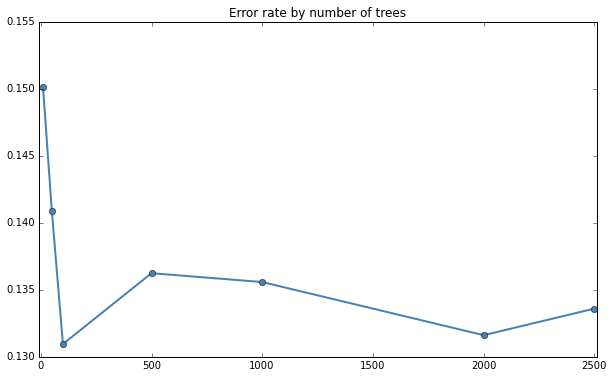
\includegraphics[scale=0.37,valign=t]{erf_vs_ntree.png}
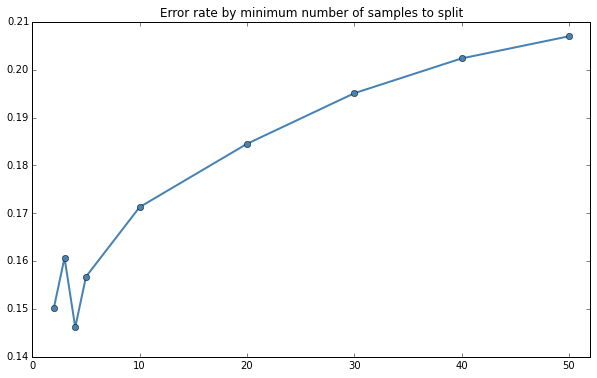
\includegraphics[scale=0.37,valign=t]{erf_vs_min_split.png}
\end{center}
\caption{Error Rate by number of estimators and minimum sample split}
\end{figure}

\noindent Figure 4.2 shows how the error rate will change when the parameters are tuned separately for ERT. The error rate in general, decreases as the number of estimator increases or the minimum sample split decreases. Moreover, using bootstrap will result in a higher rate. Using entropy (i.e. information gain) criteria resulted in a better prediction accuracy than using gini impurity for ERT. Whether each tree is warm started or not does not affect the accuracy. Finally grid search (tuning all parameters together) on ERT model has yield a $1.59\%$ decrease in the error rate when compared to the default ERT model; the best combination of parameters is: \\

\begin{table}[ht]
    \label{best_ert}
    \centering
    \begin{tabular}{c|c|c|c|c}
        \hline
        \textbf{number of estimator} & \textbf{min sample split} & \textbf{bootstrap} & \textbf{criterion} & \textbf{error} \\ \hline
        100 & 2 & False & gini & 0.1309 \\
        \hline
    \end{tabular}
    \caption{Optimal parameters for ERT}
\end{table}

\noindent Figure 4.3 shows how the error rate will change when the parameters are tuned separately for GB. Similar to ERT, as number of estimators or min sample split decreases, the error decreases. The learning rate is seems to have a quadratic relationship with the error. The error seems to be the smallest when the learning rate is around 0.4, and increases as the learning rate goes to 0 or 1. \\

\begin{figure}[ht]
\label{gb_grid}
\begin{center}
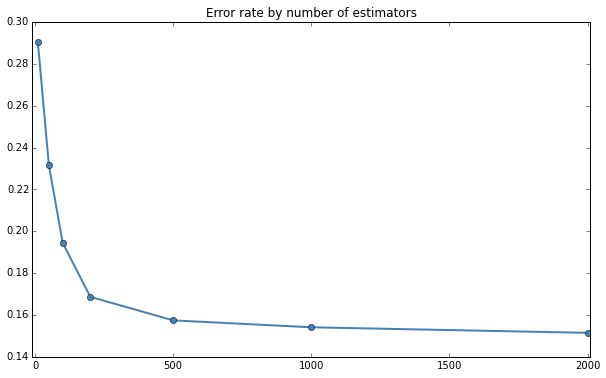
\includegraphics[scale=0.26,valign=t]{gb_vs_num_est.png}
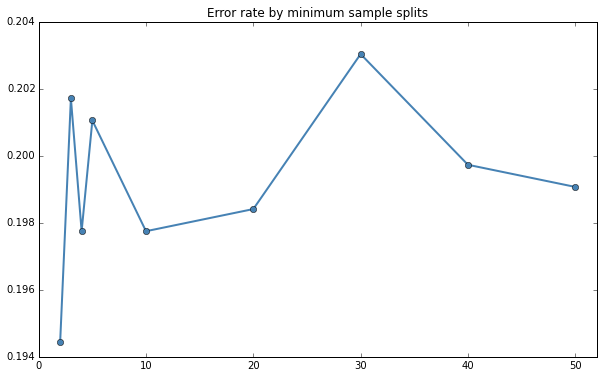
\includegraphics[scale=0.26,valign=t]{gb_vs_min_split.png}
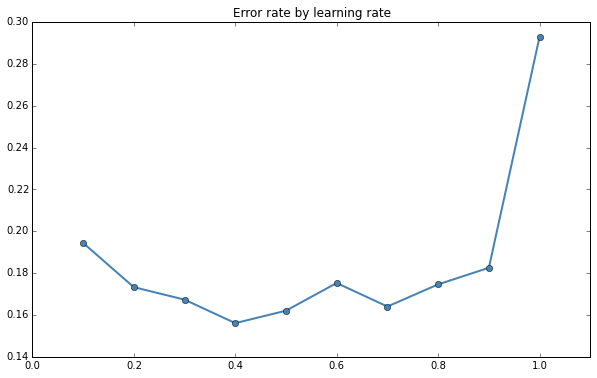
\includegraphics[scale=0.26,valign=t]{gb_vs_learning_rate.png}
\end{center}
\caption{Error Rate by number of estimators and minimum sample split. From left to right: number of estimators, min sample split, learning rate.}
\end{figure}

\noindent The best parameter combination for GB dropped the error rate by $5.42\%$ compared to the default GB model; the optimal parameter is:

\begin{table}[ht]
    \label{best_gb}
    \centering
    \begin{tabular}{c|c|c|c}
        \hline
        \textbf{number of estimator} & \textbf{min sample split} & \textbf{learning rate} & \textbf{error} \\ \hline
        2000 & 3 & 0.3 & 0.1402 \\
        \hline
    \end{tabular}
    \caption{Optimal parameters for GB}
\end{table}

\noindent In conclusion, the grid search has improved our best error rate from $14.68\%$ (ERT with default parameter) to $13.09\%$ (ERT with best parameter).

\newpage 

\subsection{Parameter Creation and Feature Selection}
Due to the limited number of features in the training data (12), we have decided to increase the number of features in order to give models more flexibility in fitting. The new features are introduced by creating the 2-way and 3-way interaction between numerical variables.\\

\noindent By including all 2-way interactions, we will result in a total of 109 features. By including all 2-way and 3-way interactions, we will result in a total of 329 features. A ERT model is fit and grid search is used to find the best parameter combinations for each case.

\begin{table}[ht]
    \label{interaction_both}
    \centering
    \begin{tabular}{c|c c c c|c}
        \hline
        \textbf{n. features} & \textbf{n. estimator} & \textbf{min sample split} & \textbf{bootstrap} & \textbf{criterion} & \textbf{error} \\ \hline
        109 & 2000 & 2 & False & gini & 0.1124 \\
        329 & 100 & 4 & False & gini & 0.1230 \\
        \hline
    \end{tabular}
    \caption{ERT on 2-way $\&$ 3-way interaction features}
\end{table}

\noindent Both models resulted in increase in prediction accuracy. For the model including all 2-way interactions, the error rate has dropped by $1.85\%$ and for the model including all 2-way and 3-way interactions, the error rate decreased by $0.79\%$.\\

\noindent Considering the possibility of having too many features in the 3-way interaction model, we used feature importance to employ feature selection. In gini criteria, the variable importance is calculated by "gini gain" produced by variable i over all trees and it is biased in favor of continuous variables and variables with many categories (Strobl $\&$ Zeileis, 2008). Figure 4.4 shows the variable importance for all 329 features in the model. By trial and error, a threshold of 0.025 has been set and all variables with an importance higher than the threshold (total of 116) were selected. The reconstructed model resulted in an error rate of 0.1197, which is a $0.33\%$ increase compared to the previous best model.

\begin{figure}[ht]
\label{feat_imp}
\begin{center}
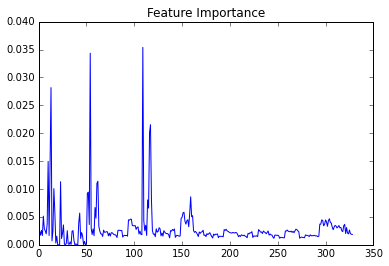
\includegraphics[scale=0.6,valign=t]{feat_imp.png}
\end{center}
\caption{Feature importance for ERT model on data with 3-way interactions.}
\end{figure}

\section{Semi-supervised Learning Methods}
Recall that we have 15,120 samples in the training set and 565,892 samples in the testing set. The training set is much smaller than the testing set and it is possible that the training set is unable to capture the underlying distribution of the complete data. We then decided to use semi-supervised learning technique to predict the cover type.\\

\noindent The idea of semi-supervised learning is to: 1) borrow unlabeled data from testing set, 2) using algorithms like label propagation and spreading to determine the label for those unlabeled data, and 3) use the expanded training set to fit model and predict on new data. \\

\noindent Figure 5.1 (extracted from Python sklearn website) shows an example of how label spreading assign labels to unlabeled data and how it prevents having wrong decision boundaries. \\

\begin{figure}[ht]
\label{label_spreading}
\begin{center}
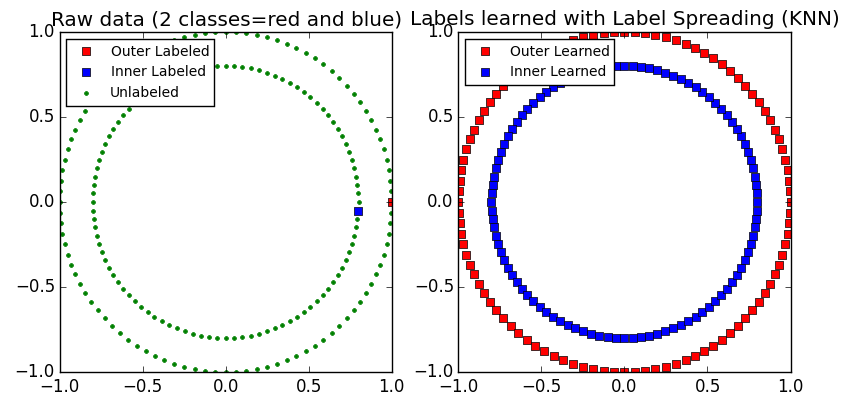
\includegraphics[scale=0.6,valign=t]{semi_sup.png}
\end{center}
\caption{Label spreading method in semi-supervised learning.}
\end{figure}

\subsection{Parameters in Label Propagation / Spreading}
Both label propagation and label spreading are graph-based learning methods. They use a graph representation of the data and represent them like a network with nodes and edges. In this way, the similarity measurements are easier. Label propagation uses the raw similarity matrix constructed from the data with no modifications whereas label spreading minimizes a loss function that has regularization properties which is more robust to noise. Label spreading, on each iteration, modifies the original matrix and calculate the normalized graph Laplacian matrix for updates (Scikit-Learn, 2015). \\

\noindent Both models have clamping parameters and choice of kernel functions. Clamping parameters allows the algorithm to change the weight of the true ground labeled data distribution to some degree ($\alpha$ level). For kernel functions, RBF and KNN can be selected. Due to the memory consuming of RBF kernel, only KNN model has been fit. \\

\noindent We have also selected different percentages of testing data to borrow to determine model accuracy. The rate chosen are: $5\%$, $10\%$ and $20\%$. $50\%$ and $100\%$ borrow rates were also tested at the end to see how the result compares on Kaggle leader board. \\

\noindent Moreover, by initial training of label propagation, we noticed that the algorithm is changing approximately $20\%$ the original label of the training data. Considering those are the absolutely correct labels, we manually changed them back.

\noindent During this section, only Extremely Randomized Trees model with default parameters and 1000 estimators is fit to examine the error rate. \\

\subsection{Model Fitting Result}

Table 5.1 shows the result from each scenario. We noticed that the error rate decreases as we borrow more data from the testing set. Hard clamping ($\alpha$=1) gave the best result among all choice of $\alpha$'s.

\begin{table}[ht]
    \label{semi_sub_result}
    \centering
    \begin{small}
    \begin{tabular}{c c|c|c}
        \hline
        \textbf{$\%$ test data borrowed} & \textbf{alpha} & \textbf{Label spreading test error} & \textbf{Label propagation test error} \\ \hline
        $5\%$ & 1.0 & 0.1865 & 0.1852 \\
        $5\%$ & 0.8 & 0.1865 & 0.1909 \\
        $5\%$ & 0.6 & 0.1889 & 0.2015 \\
        $10\%$ & 1.0 & 0.1386 & 0.1403 \\
        $10\%$ & 0.8 & 0.1534 & 0.1527 \\
        $10\%$ & 0.6 & 0.1590 & 0.1692 \\
        $20\%$ & 1.0 & 0.0959 & 0.0969 \\
        $20\%$ & 0.8 & 0.1062 & 0.1058 \\
        $20\%$ & 0.6 & 0.1101 & 0.1183 \\
        \hline
    \end{tabular}
    \end{small}
    \caption{Testing error of ERT on label propagated / spread data}
\end{table}

\subsection{judgement on Error Rate}

However, recall that in the training set, approximately 80$\%$ (15120 / (15120 + 565892)) of the data are from the testing set. Those borrowed data are assigned labels using label spreading or propagation algorithm with KNN kernel, and we do not know whether the assigned labels are correct or not. In other words, the training data is not $100\%$ accurate. Though the test error decreased, we cannot conclude that the test error represents the true error in the testing set.

\newpage

\section{Kaggle Ranking Result}

All the models discussed previously were submitted on Kaggle and retrieved true testing error, which is shown in Table 6.1. Figure 6.1 shows the distribution of the scores on Kaggle. \\

\begin{table}[ht]
    \label{kaggle_result}
    \centering
    \begin{small}
    \begin{tabular}{|>{\centering\arraybackslash}m{3in}|>{\centering\arraybackslash}m{1in}|>{\centering\arraybackslash}m{2in}|}
        \hline
        \textbf{Model} & \textbf{Score} & \textbf{Ranking (out of 1694 teams)} \\ \hline
        ERT + raw data & 0.75793 & 591  \\ \hline
        GB + raw data & 0.72622 & 1074  \\ \hline
        ERT + 2-way interaction & 0.77803 & 368  \\ \hline
        ERT + 3-way interaction & 0.75972 & 540  \\ \hline
        \textcolor{green}{ERT + 3-way interaction + feature selection} & \textcolor{green}{0.77985} & \textcolor{green}{362}  \\ \hline
        semi-sup label spreading + raw data + 20$\%$ borrow rate + $\alpha=1$ + ERT & 0.65952 & 1349  \\ \hline
        semi-sup label spreading + raw data + 50$\%$ borrow rate + $\alpha=1$ + ERT & 0.73131 & 1022  \\ \hline
        semi-sup label spreading + 2-way interaction data + 20$\%$ borrow rate + $\alpha=1$ + ERT & 0.73135 & 1022  \\ \hline
        semi-sup label spreading + 2-way interaction data + 100$\%$ borrow rate + $\alpha=1$ + ERT & 0.77320 & 395  \\
        \hline
    \end{tabular}
    \end{small}
    \caption{Kaggle score and ranking}
\end{table}

\begin{figure}[ht]
\label{kaggle_rank}
\begin{center}
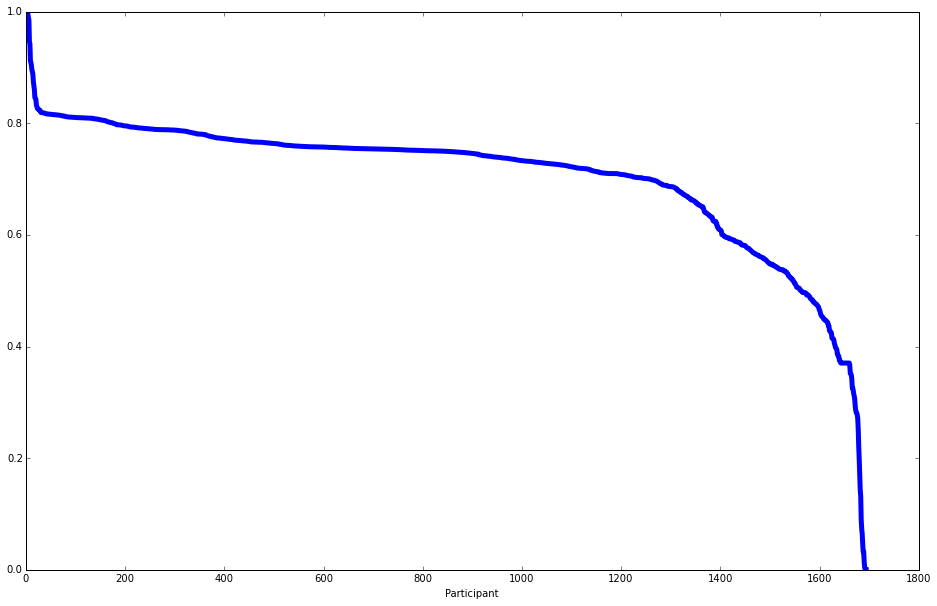
\includegraphics[scale=0.3,valign=t]{kaggle.png}
\end{center}
\caption{Kaggle ranking distribution.}
\end{figure}




\section{Conclusion}
By applying supervised and semi-supervised machine learning algorithms, using grid search, feature creation and selection techniques, we are able to predict the predominant forest cover type in this Kaggle competition and rank top 20$\%$ among all the competitors. The best performing model is the extremely randomized tree model with grid searched parameters fitting on data with 116 features selected from features including base, 2-way and 3-way interactions by gini variable importance.


\newpage

\section{Supplementary Material}
All related files are uploaded to Github \href{https://github.com/zhangyilun/stat441project}{https://github.com/zhangyilun/stat441project}. The related folders/files are
\begin{itemize}
\item "data/" contains the raw data and transformed data
\item "plot/", "trans\_no/", "trans\_yes/" contain some of the plots generated and used in the report
\item "submission/" contains all the files submitted to Kaggle
\item "\textbf{model.ipynb}" contains majority of the code used for EDA and supervised model fitting
\item "\textbf{semi\_s\_model.ipynb}" contains majority of the code used for fitting semi-supervised learning models
\item "*.py" contains the code to fit models and running from command line due to IPython kernel dead.
\end{itemize}


% references
\def\bibindent{1em}
\begin{thebibliography}{99\kern\bibindent}
\makeatletter
\let\old@biblabel\@biblabel
\def\@biblabel#1{\old@biblabel{#1}\kern\bibindent}
\let\old@bibitem\bibitem
\def\bibitem#1{\old@bibitem{#1}\leavevmode\kern-\bibindent}
\makeatother

% example
% \textsc{A. Paula Palacios, J. Miguel Marín, Emiliano J. Quinto, and Michael P. Wiper. (2014). \href{http://arxiv.org/pdf/1411.5780.pdf}{Bayesian modeling of bacterial growth for multiple populations}. \textit{Ann. Appl. Stat.}, Volume 8, Number 3, 1516-1537.}\\
% [0.2cm]

\textsc{Kaggle: The Home of Data Science. (2015). Description - Forest Cover Type Prediction, Kaggle. Retrieved on Dec 7th, 2015 from: \href{https://www.kaggle.com/c/forest-cover-type-prediction}{\texttt{https://www.kaggle.com/c/forest-cover-type-prediction}}.}\\
[0.2cm]

\textsc{Wikipedia. (2015). Principal component analysis. Retrieved on Dec 7th, 2015 from: \href{https://en.wikipedia.org/wiki/Principal_component_analysis}{\texttt{https://en.wikipedia.org/wiki/Principal\_component\_analysis}}.}\\
[0.2cm]

\textsc{Wikipedia. (2015). Linear discriminant analysis. Retrieved on Dec 7th, 2015 from: \href{https://en.wikipedia.org/wiki/Linear_discriminant_analysis}{\texttt{https://en.wikipedia.org/wiki/Linear\_discriminant\_analysis}}.}\\
[0.2cm]

\textsc{Scikit-Learn. (2015). Ensemble methods. Retrieved on Dec 7th, 2015 from: \href{http://scikit-learn.org/stable/modules/ensemble.html}{\texttt{http://scikit-learn.org/stable/modules/ensemble.html}}.}\\
[0.2cm]

\textsc{Scikit-Learn. (2015). Semi-supervised. Retrieved on Dec 7th, 2015 from: \href{http://scikit-learn.org/stable/modules/label_propagation.html}{\texttt{http://scikit-learn.org/stable/modules/label\_propagation.html}}.}\\
[0.2cm]

\textsc{H. D. Laura. (2014). Machine Learning Algorithm. Retrieved on Dec 7th, 2015 from: \href{http://www.lauradhamilton.com/machine-learning-algorithm-cheat-sheet}{\texttt{http://www.lauradhamilton.com/machine-learning-algorithm-cheat-sheet}}.}\\
[0.2cm]

\textsc{R. Thomas. (2015). Adaboost Algorithm, MIT. Retrieved on Dec 7th, 2015 from: \href{http://math.mit.edu/~rothvoss/DiscreteMath3PMSpring2013.html}{\texttt{http://math.mit.edu/~rothvoss/DiscreteMath3PMSpring2013.html}}.}\\
[0.2cm]

\textsc{S. Carolin, Z. Achim. (2008). Why and how to use random forest variable importance measures (and how you shouldn't). Retrieved on Dec 7th, 2015 from: \href{http://www.statistik.uni-dortmund.de/useR-2008/slides/Strobl+Zeileis.pdf}{\texttt{http://www.statistik.uni-dortmund.de/useR-2008/slides/Strobl+Zeileis.pdf}}. }\\
[0.2cm]

\end{thebibliography}
\end{document}
